\documentclass{beamer}
\usepackage[T1]{fontenc}
\usepackage{lmodern}
\usepackage{amsmath}
\usepackage{amsfonts}
\usepackage{amssymb}
\usepackage{amsthm}
\usepackage{graphicx}
\usepackage{color}
\usepackage{xcolor}
\usepackage{url}
\usepackage{textcomp}
\usepackage{parskip}
\usetheme{Pittsburgh}


\usepackage{multicol}
\setlength{\columnsep}{1cm}

\graphicspath{ {Images/} }

\beamertemplatenavigationsymbolsempty

\title{Introduction à l'analyse des réseaux sociaux}
\subtitle{MSH Lyon / Saint-Etienne}
\author{Maxime Cornet - Institut Polytechnique de Paris}
\date{27 Octobre 2021}
\begin{document}

\begin{frame}
    \titlepage
\end{frame}

\begin{frame}
    \frametitle{Introduction:}
    \begin{enumerate}[I]
        \item Qu'est ce qu'un réseau? Terminologie \& Théorie des graphes
        \item Pourquoi étudier la structure des interactions? Origine du concept
        \item Calculs \& métriques de base
        \item Exemples d'application
    \end{enumerate}
\end{frame}

\begin{frame}
    \frametitle{I) Qu'est-ce qu'un réseau social?}
\begin{center}
    \begin{quotation}
        « l’analyse des réseaux sociaux est un ensemble de sous méthodes pour analyser des ensembles de relations sociales, considérées elles-mêmes comme émergeant des interactions entre des personnes ou des groupes »
    \end{quotation}
    - Degenne, Forsé, 1994
\end{center}
\end{frame}

\begin{frame}
    \frametitle{I) Qu'est-ce qu'un réseau social?}
\begin{itemize}
    \item Un outil d'analyse
    \item Prise en compte de l’intégralité des relations interactionnelles données, pour observer la structure relationnelle qui émerge de ces relations
    \item Dans une temporalité propre 
    \item Survenant dans un contexte délimité
\end{itemize}
\end{frame}

\begin{frame}
    \frametitle{I) Comment ça se formalise?}
    \begin{figure}
        \centering
        \includegraphics[width = 0.7\textwidth]{network_exemple.png}
        \caption{\small{Exemple de réseau}}
    \end{figure}
\end{frame}

\begin{frame}
    \frametitle{I) Comment ça se formalise?}
    \begin{figure}
        \centering
        \includegraphics[width = 0.9\textwidth]{network_exemple_matrix.png}
        \caption{\small{Matrice du réseau vu en slide précédente}}
      \end{figure}
\end{frame}

\begin{frame}
    \frametitle{I) L'analyse de réseaux}
    \begin{itemize}
        \item Théorie des graphes: une branche des mathématiques remontant au « problème des sept ponts de Konigsberg » d’Euler.
        \item Noeuds (nodes): vertex; acteurs
        \item Arrête (edge): arcs; liens; relations
        \item Plusieurs types: réseaux complets; réseaux personnels réseaux techniques 
        \item  Plusieurs formes: dirigés / non dirigés; one-mode / two mode
    \end{itemize}
\end{frame}

\begin{frame}
    \frametitle{I) Reseaux dirigés}
    \begin{figure}
        \centering
        \includegraphics[width = 0.7\textwidth]{exemple_graphes_dirige.png}
        \caption{\small{Exemple de réseau dirigé}}
    \end{figure}
\end{frame}

\begin{frame}
    \frametitle{I) Réseaux dirigés}
    \begin{figure}
        \centering
        \includegraphics[width = 0.9\textwidth]{exemple_graphe_dirige_matrice.png}
        \caption{\small{Matrice du réseau vu en slide précédente}}
      \end{figure}
\end{frame}

\begin{frame}
    \frametitle{I) Collecter des donnees de reseau}
    \begin{itemize}
        \item Variabilité des sources (webscrapping, questionnaire, entretiens, archives)
        \item Variabilité des modes de collecte (rappel libre, liste à coche, sociogramme, etc.)
        \item Biais attendus et spécifiques aux dispositif de collecte
        \item Attention aux données manquantes: problèmes spécifique pour les données de réseau.
    \end{itemize}
\end{frame}

\begin{frame}
    \frametitle{I) Délimiter un réseau}
    \begin{itemize}
        \item Le réseau résulte d'un ensemble de décisions méthodologiques qui doivent être prises consciemment en rapport avec les hypothèses de départ.
        \item Qui sont les noeuds? Quelles interactions relever?
        \item Ou commence et s'arrête le réseau? Spatialement et temporellement?
        \item L'analyse de la structure n'a de sens qu'en gardant ces aspects méthodologiques et réflexifs en tête.
    \end{itemize}
\end{frame}

\begin{frame}
    \frametitle{II) Une structure qui émerge des intéractions?}
    \begin{itemize}
        \item Georg Simmel (1905): la triade est l’unité
        d’analyse fondamentale en sociologie. 
        \item La dynamique sociale de trois acteurs dans une triade est qualitativement différente de ce qui est issu de l’observation d’une dyade ou d’un individu isolé.
        \item Les comportements et phénomènes sociaux ne peuvent pas être réduits à des dyades ou individus.
    \end{itemize}
\end{frame}

\begin{frame}
    \frametitle{II) Méthodes anciennes}
    \begin{columns}
        \begin{column}{0.5\textwidth}
            \begin{figure}
                \centering
                \includegraphics[width = \textwidth]{moreno_sociogramme.png}
            \end{figure}
        \end{column}
        \begin{column}{0.5\textwidth}
            Première représentation que l'on connaît (celle en graphe), on la doit à Moreno: lLe sociogramme. - Moreno, 1938
        \end{column}
    \end{columns}
\end{frame}

\begin{frame}
    \frametitle{II) Dynamiques sociales}
    \begin{itemize}
        \item J. A. Barnes (1955): S'appuie en partie sur les travaux de Moreno, et introduit la notion de "réseau", et la notion de multiplicité de réseau entremêlés. 
        \item "I find it convenient to talk of a social field of this kind as a network (...) We can of course thinks of the whole of social life as generating a network of this kind".
        \item "So far we have looked at Bremnes society as an isolated object of study. (... ) In reality, Bremnes is not an isolated society, and there is the large descriptive and analytical problem of understanding the relationship between bremnes and neighbouring parishes, and between it and the Norwegian state."
    \end{itemize}
\end{frame}

\begin{frame}
    \frametitle{II) Etudier les interactions}
    Abbott (1997, 2001): Les théories sociologiques s’intéressent aux
    acteurs et à leurs interactions, alors que les méthodes sociologiques s’intéressent aux variables et à leurs interactions .Il y a là une incohérence entre théorie et méthode, qui ne peuvent pas se nourrir l’une l’autre.
\end{frame}

\begin{frame}
    \frametitle{II) Transitivité:}
    \begin{figure}
        \centering
        \includegraphics[width = 0.9\textwidth]{triades_transitivite.png}
      \end{figure}
\end{frame}

\begin{frame}
    \frametitle{II) Nature dynamique des intéractions:}
    \begin{itemize}
        \item La plupart des réseaux sociaux observés empiriquement ont un degré élevé de transitivité. (Beaucoup plus elevé que dans les réseaux aléatoires)
        \item La transitivité est une caractéristique essentielle des relations humaines : les êtres humains se lient entre eux par des intermédiaires.
        \item Granovetter (1973): La triade intransitive est instable, on peut prédire qu’un lien se formera par transitivité tôt ou tard.
    \end{itemize}
\end{frame}

\begin{frame}
    \frametitle{III) Métriques structurelles et définitions: globales}
    \begin{itemize}
        \item Densité: Mesurer la cohésion (globale) : Le rapport entre le nombre de liens qui existent et ceux qui pourraient exister.
        \item Diamètre: la distance entre deux nœuds les plus distants dans un réseau.
        \item Distance moyenne: distance moyenne entre toutes les paires de nœuds.
        \item Rayon:  la plus petite distance à laquelle puisse se trouver un nœud de tous les autres.
    \end{itemize}
\end{frame}

\begin{frame}
    \frametitle{III) Métriques structurelles et définitions: globales}
    \begin{itemize}
        \item Transitivité: L’indice de transitivité globale d’un réseau: nombre triades transitives / nombre triades.
        \item Il est égal à 1 si tous les nœuds sont liés à tous les autres nœuds (connectivité complète).
        \item Dans des réseaux aléatoires, il excède rarement 0.2. Dans les réseaux empiriques, il est souvent compris entre 0.3 et 0.6
        \item Variante locale: Le coefficient de clustering (ou coefficient d’agglomération), est une mesure de la cohésion dans le voisinage d’un nœud (combien de mes amis sont amis entre eux).
    \end{itemize}
\end{frame}

\begin{frame}
    \frametitle{III) Métriques structurelles et définitions:}
    \begin{itemize}
        \item Réciprocité: dans les réseaux dirigés, taux de liens qui vont dans les deux sens.
        \item Nombre de cliques: Une clique est un sous-ensemble de nœuds où toutes les paires de nœuds existants sont connectées. (ex: d'implication structurelles:  Co-appartenance comme indicateur de cohésion; Alba \& Kadushin, 1976). Taille moyenne des cliques et plus grande clique.
        \item Excentricité: la distance depuis un nœud de départ vers le nœud le plus loin dans le réseau.
    \end{itemize}
\end{frame}

\begin{frame}
    \frametitle{III) Centralité:}
    \begin{itemize}
        \item On tente de répondre à la question, quel rôle occupe quel noeud dans le réseau? -> Calcul de propriétés structurelles des noeuds.
        \item Les acteurs ont des caractéristiques propres, qui dépendent de la structure globale du réseau et de leur positon dans celle ci.
        \item Plusieurs types de centralité, à mobiliser en fonction des hypothèses de départ.
    \end{itemize}
\end{frame}

\begin{frame}
    \frametitle{III) Centralité de degrés:}
    \begin{itemize}
        \item Centralité de degré: Qui sont les nœuds les plus « actifs »? On compte tour simplement le nombre de lien qui relient un noeud à d'autres.
        \item !Comparaisons de centralité possible seulement si les réseaux sont de même taille : degré = 8 veut dire être connecté à 80\% s’il y a 10 acteurs, à 20\% s’il n’y en a que 40. (utiliser le calcul normalisé)
        \item Degré entrant / sortants: pour les graphes connectés: nombre de liens émis / reçus.
    \end{itemize}
\end{frame}

\begin{frame}
    \frametitle{III) Centralité:}
    \begin{figure}
        \centering
        \includegraphics[width = 0.5\textwidth]{degres.png}
        \caption{\small{Centralité de degrés. Rouge = plus élevée. source: wikipédia}}
      \end{figure}
\end{frame}

\begin{frame}
    \frametitle{III) Centralité d’intermédiarité:}
    \begin{itemize}
        \item La centralité d’intermédiarité identifie les gatekeepers dans le réseau. Davantage de chemins passent par ces acteurs, qui peuvent passer l’information à d’autres dans le réseau (ou la stopper).
        \item La centralité d’intermédiarité est parfois une mesure plus pertinente de l’« importance » dans un réseau. Les acteurs avec plus grande centralité d’intermédiarité: \begin{itemize}
            \item Connectent des groupes différents dans un réseau, et constituent parfois le seul lien entre eux
            \item Contrôlent les flux de communication dans le réseau
            \item Peuvent agir en intermédiaires
        \end{itemize}
        \item Calcul: Il faut prendre en compte non seulement les liens directs de l’acteur i, mais tout le réseau. On compte le nombre de plus courts chemins entre toute paire d’acteurs k et j, et on prend ceux qui passent par i.
    \end{itemize}
\end{frame}

\begin{frame}
    \frametitle{III) Centralité:}
    \begin{figure}
        \centering
        \includegraphics[width = 0.5\textwidth]{intermediarite.png}
        \caption{\small{Centralité d'intermédiarité. Rouge = plus élevée. source: wikipédia}}
      \end{figure}
\end{frame}

\begin{frame}
    \frametitle{III) Centralité de vecteur propre (eigenvalue):}
    \begin{itemize}
        \item Vecteur propre: Donne plus de poids aux acteurs avec le plus grand nombre de liens. Mais elle donne un poids plus élevé aux contacts qui sont eux-mêmes centraux dans le réseau.
        \item Elle effectue une pondération des contacts sur la base de leur centralité. Ce faisant, elle tient compte de la structure du réseau dans son ensemble.
        \item La centralité eigenvector peut être vue comme une version récursive de la centralité de degré : \begin{enumerate}
            \item Commencez en assignant centralité 1 à tous les nœuds
            \item Recalculez le résultat pour chaque nœud comme somme pondérée des centralités de tous les nœuds dans son voisinage.
            \item Normalisez en divisant chaque valeur par le maximum
            \item Répétez les étapes 2 et 3 jusqu’à ce que les valeurs arrêtent de changer.
        \end{enumerate}
    \end{itemize}
\end{frame}

\begin{frame}
    \frametitle{III) Centralité:}
    \begin{figure}
        \centering
        \includegraphics[width = 0.5\textwidth]{vecteur_propre.png}
        \caption{\small{Centralité de vecteur propre. Rouge = plus élevée. source: wikipédia}}
      \end{figure}
\end{frame}

\begin{frame}
    \frametitle{III) Centralisation:}
    \begin{itemize}
        \item Dans quelle mesure le réseau est dominé par un nœud central (ou peu de nœuds centraux)?
        \item On compare la centralité du nœud le plus central à la centralité des autres nœuds. On normalise en divisant par la centralité maximale d’un réseau de la même taille.
        \item Le résultat varie entre 0 et 1 (réseau en étoile). Elle tends à varier dans le temps.
    \end{itemize}
\end{frame}

\begin{frame}
    \frametitle{IV) Quelques exemples d'usage des réseaux:}
    \begin{columns}
        \begin{column}{0.5\textwidth}
            \begin{figure}
                \centering
                \includegraphics[width = \textwidth]{granovetter_getting_a_job.png}
            \end{figure}
        \end{column}
        \begin{column}{0.5\textwidth}
            \begin{itemize}
                \item Granovetter (1973, 1974): importance des relations pour trouver un emploi
                \item Liens forts moins efficaces que liens faibles
                \item Un défi pour la théorie sociologique de l’époque, qui insistait sur les bienfaits de la cohésion
            \end{itemize}
        \end{column}
    \end{columns}
\end{frame}


\begin{frame}
    \frametitle{IV) Quelques exemples d'usage des réseaux:}
    \begin{itemize}
        \item Conceptuellement, Granovetter étudie les chaînes d'accès à une ressources mobilisées par un acteur, en les contextualisant grâce à son réseau personnel
        \item Notion liens forts / liens faibles: attributs des liens, ici liés à la fréquence de l'interaction.
        \item Nombreuses décisions en lien avec les théories mobilisées par Granovetter: réseaux personnels, chaîne interactionnelles, etc.
    \end{itemize}
\end{frame}

\begin{frame}
    \frametitle{IV) Quelques exemples d'usage des réseaux:}
    \begin{itemize}
        \item Martina Morris (1995): étudie la diffusion du VIH dans les années 90, en particulier les effets de différentes "\emph{culturally specific sexual network structure}" sur la diffusion du virus.
        \item Elle trouve que la forte présence de relations co-occurentes dans un réseau réduis la probabilité de survenue d'une vague épidémique, mais augmente fortement la diffusion en cas de survenue, par rapport à la monogamie séquentielle. 
        \item Elle trouve aussi que la configuration "dissortative", ou les noeuds les plus actifs ont des relations avec les noeuds les moins actifs est la plus favorable à la diffusion du virus.
    \end{itemize}
\end{frame}

\begin{frame}
    \frametitle{IV) Quelques exemples d'usage des réseaux:}
    \begin{columns}
        \begin{column}{0.5\textwidth}
            \begin{figure}
                \centering
                \includegraphics[width = \textwidth]{Morris.png}
            \end{figure}
        \end{column}
        \begin{column}{0.5\textwidth}
            \begin{itemize}
                \item Importance de croiser les mesures
                \item Le taux de co-occurence des relations est le même dans les deux réseaux, mais les schémas de diffusion sont très différents
            \end{itemize}
        \end{column}
    \end{columns}
\end{frame}

\begin{frame}
    \frametitle{IV) Quelques exemples d'usage des réseaux:}
    \begin{itemize}
        \item Morris travaille sur des modèles relationnels de diffusion: ce ne sont pas des réseaux empiriques, mais des réseaux simulés.
        \item Les paramètres des modèles sont tirés d'études réelles, mais la structure relationnelle est entièrement artificielle.
        \item Morris utilise ces différents modèles de structure pour tester des hypothèses de diffusion. Elle définis aussi les sous-structures qui lui semblent importante pour tester ses hypothèses.
    \end{itemize}
\end{frame}

\begin{frame}
    \frametitle{IV) Quelques exemples d'usage des réseaux:}
    \begin{itemize}
        \item Gaumont, Panahi, Chavalarias (2018): Étudient les réseaux socio-sémantiques politiques du twitter francophone pendant l'élection présidentielle française de 2017.
        \item Se focalisent sur les retweet de comptes politiques, et en infèrent une appartenance politique.
        \item Ils étudient la manière dont la structure du réseau de diffusion sur twitter évoluent durant toute la campagne. Ils traitent donc de l'aspect évolutif et longitudinal des réseaux.
    \end{itemize}
\end{frame}

\begin{frame}
    \frametitle{IV) Quelques exemples d'usage des réseaux:}
    \begin{figure}
        \centering
        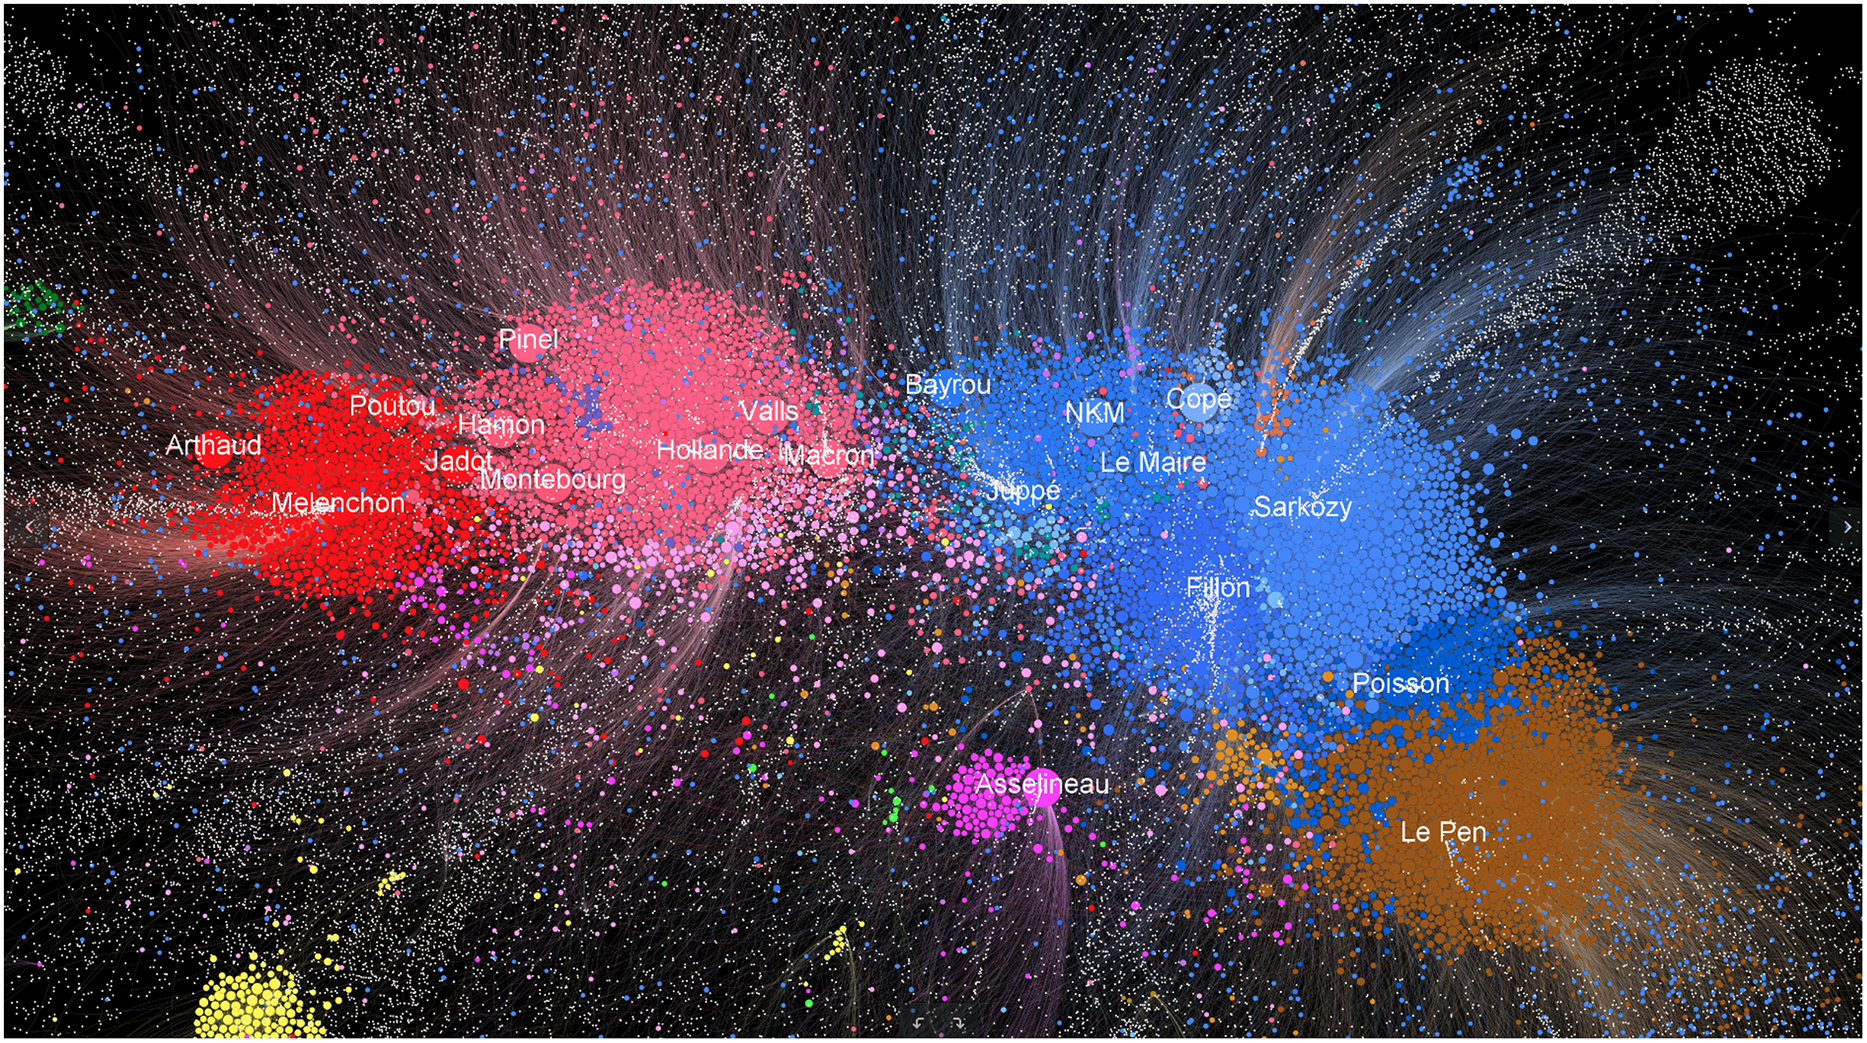
\includegraphics[width = \textwidth]{Chavalarias_fig_1.png}
        \caption{\small{Avant le début de la campagne}}
      \end{figure}
\end{frame}

\begin{frame}
    \frametitle{IV) Quelques exemples d'usage des réseaux:}
    \begin{figure}
        \centering
        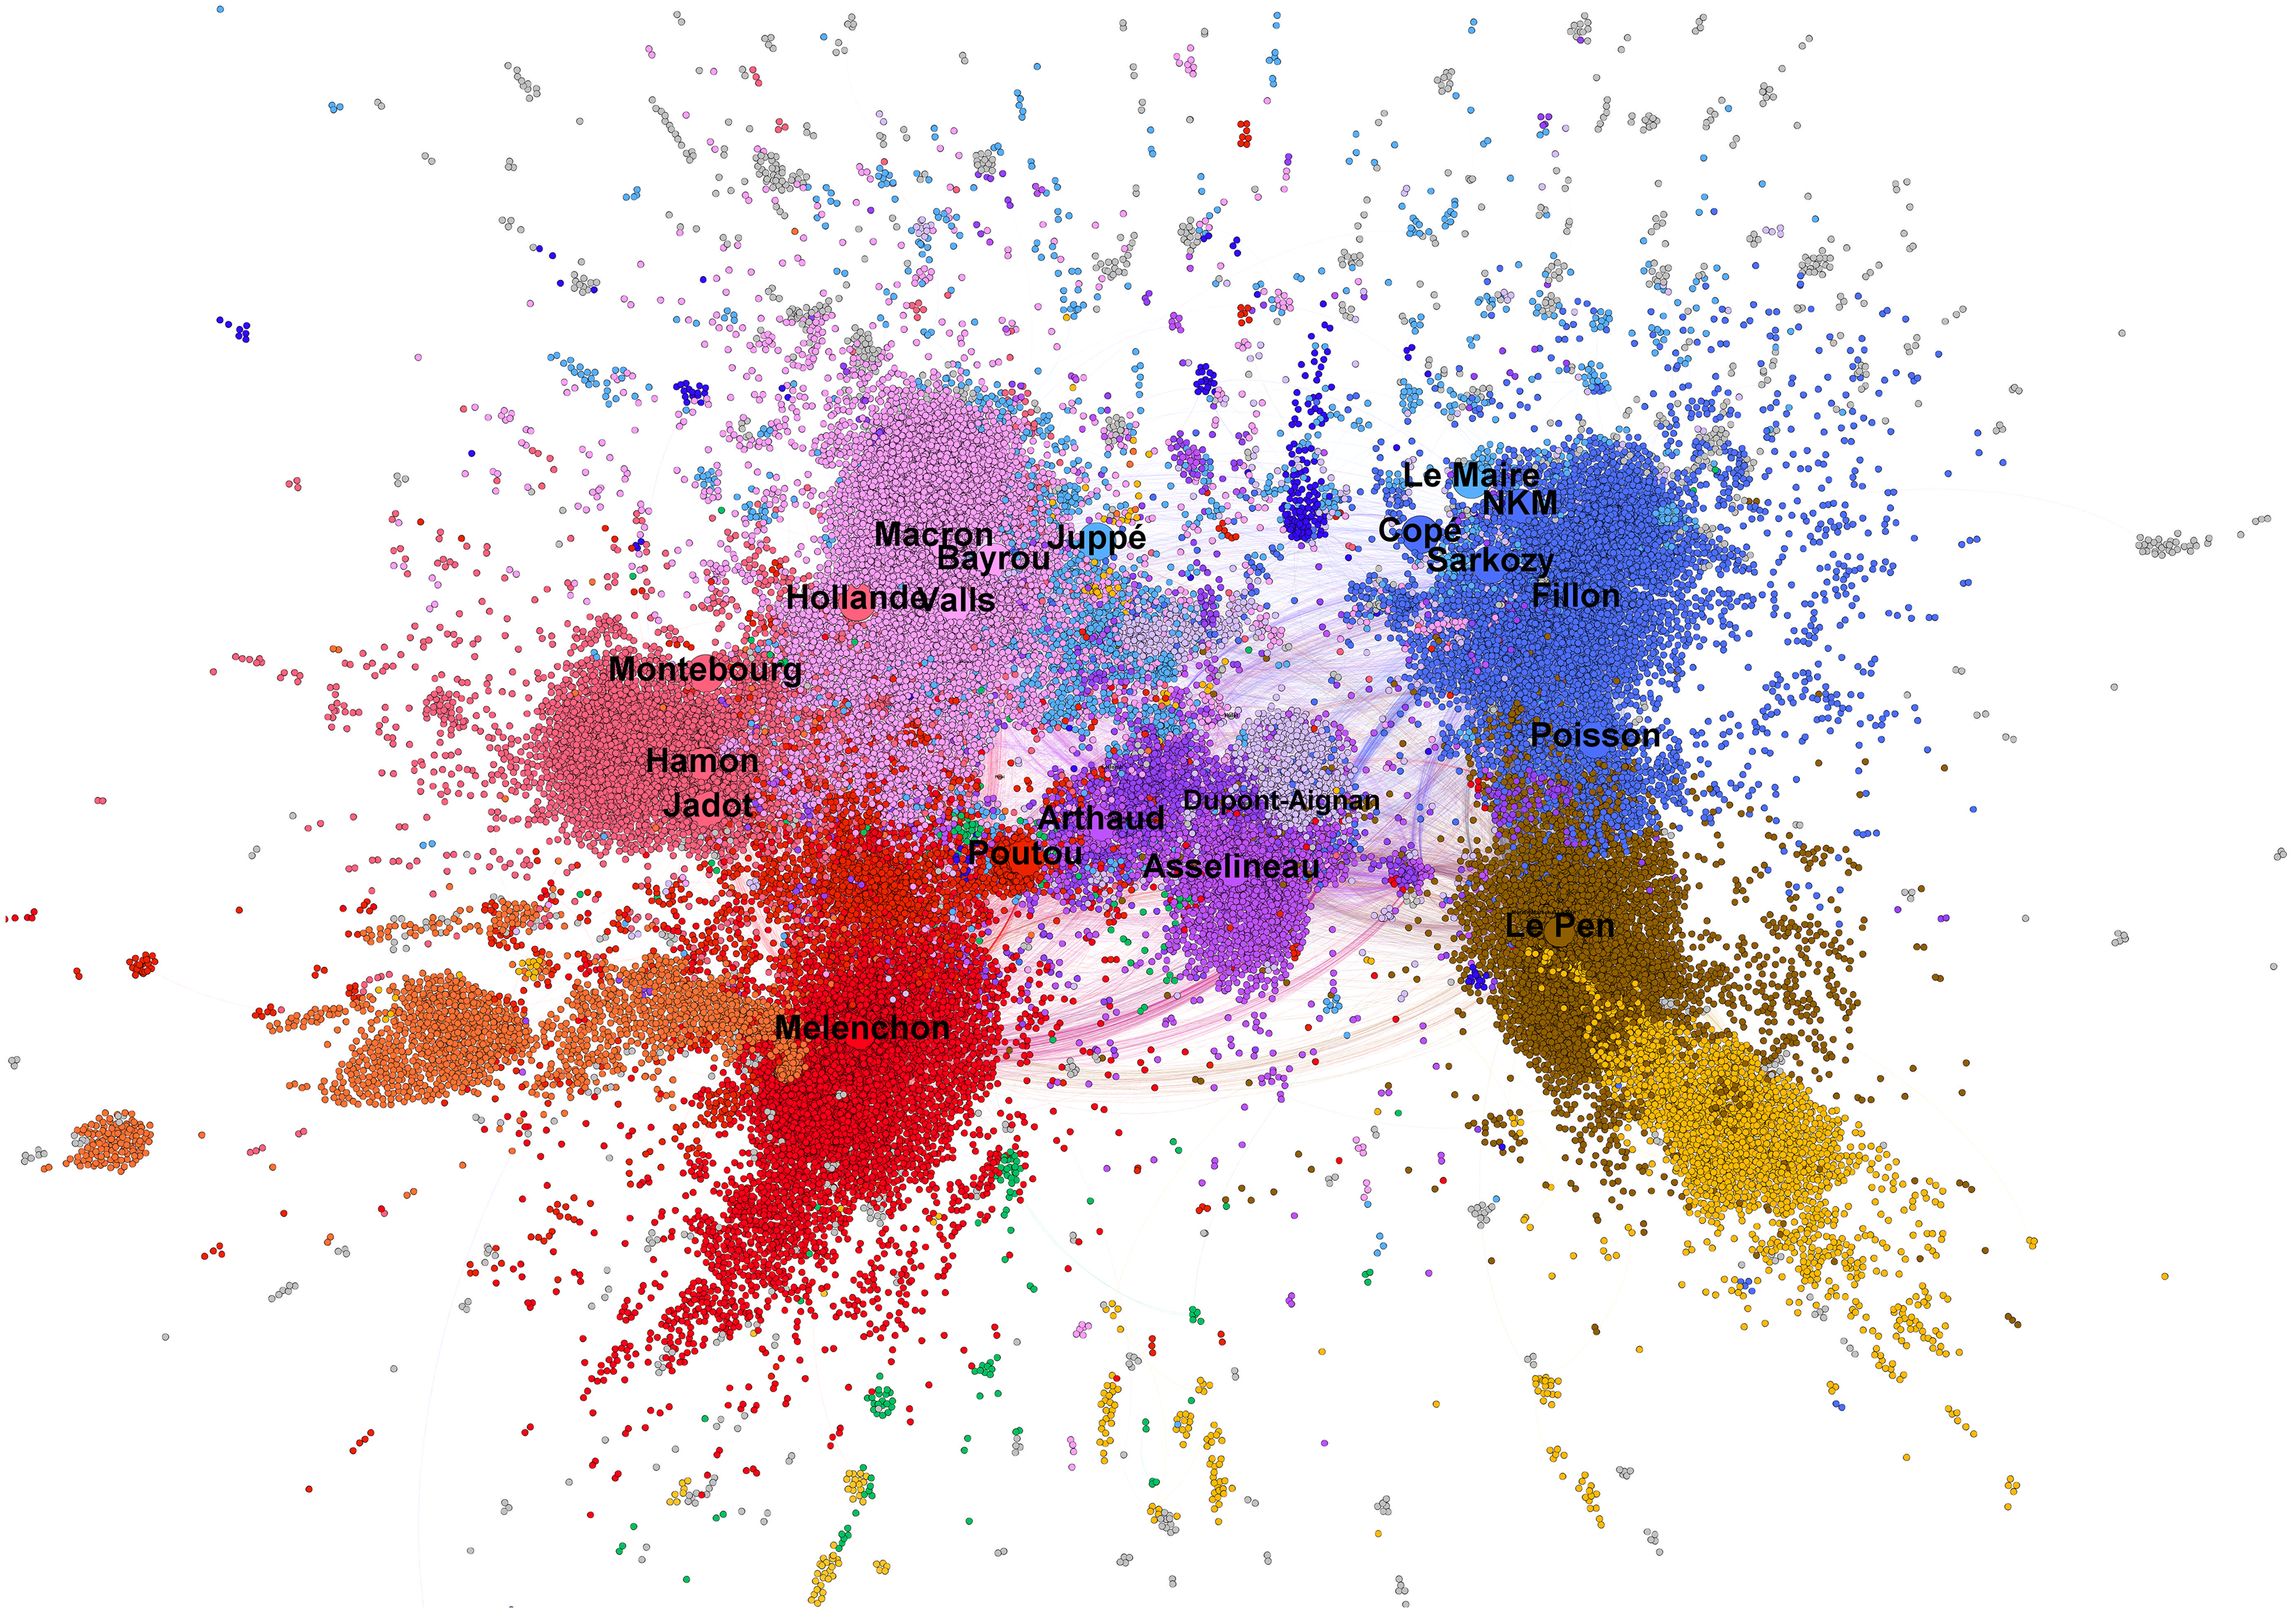
\includegraphics[width = 0.8\textwidth]{Chavalarias_fig_2.png}
        \caption{\small{Avant le premier tour}}
      \end{figure}
\end{frame}

\begin{frame}
    \frametitle{IV) Quelques exemples d'usage des réseaux:}
    \begin{figure}
        \centering
        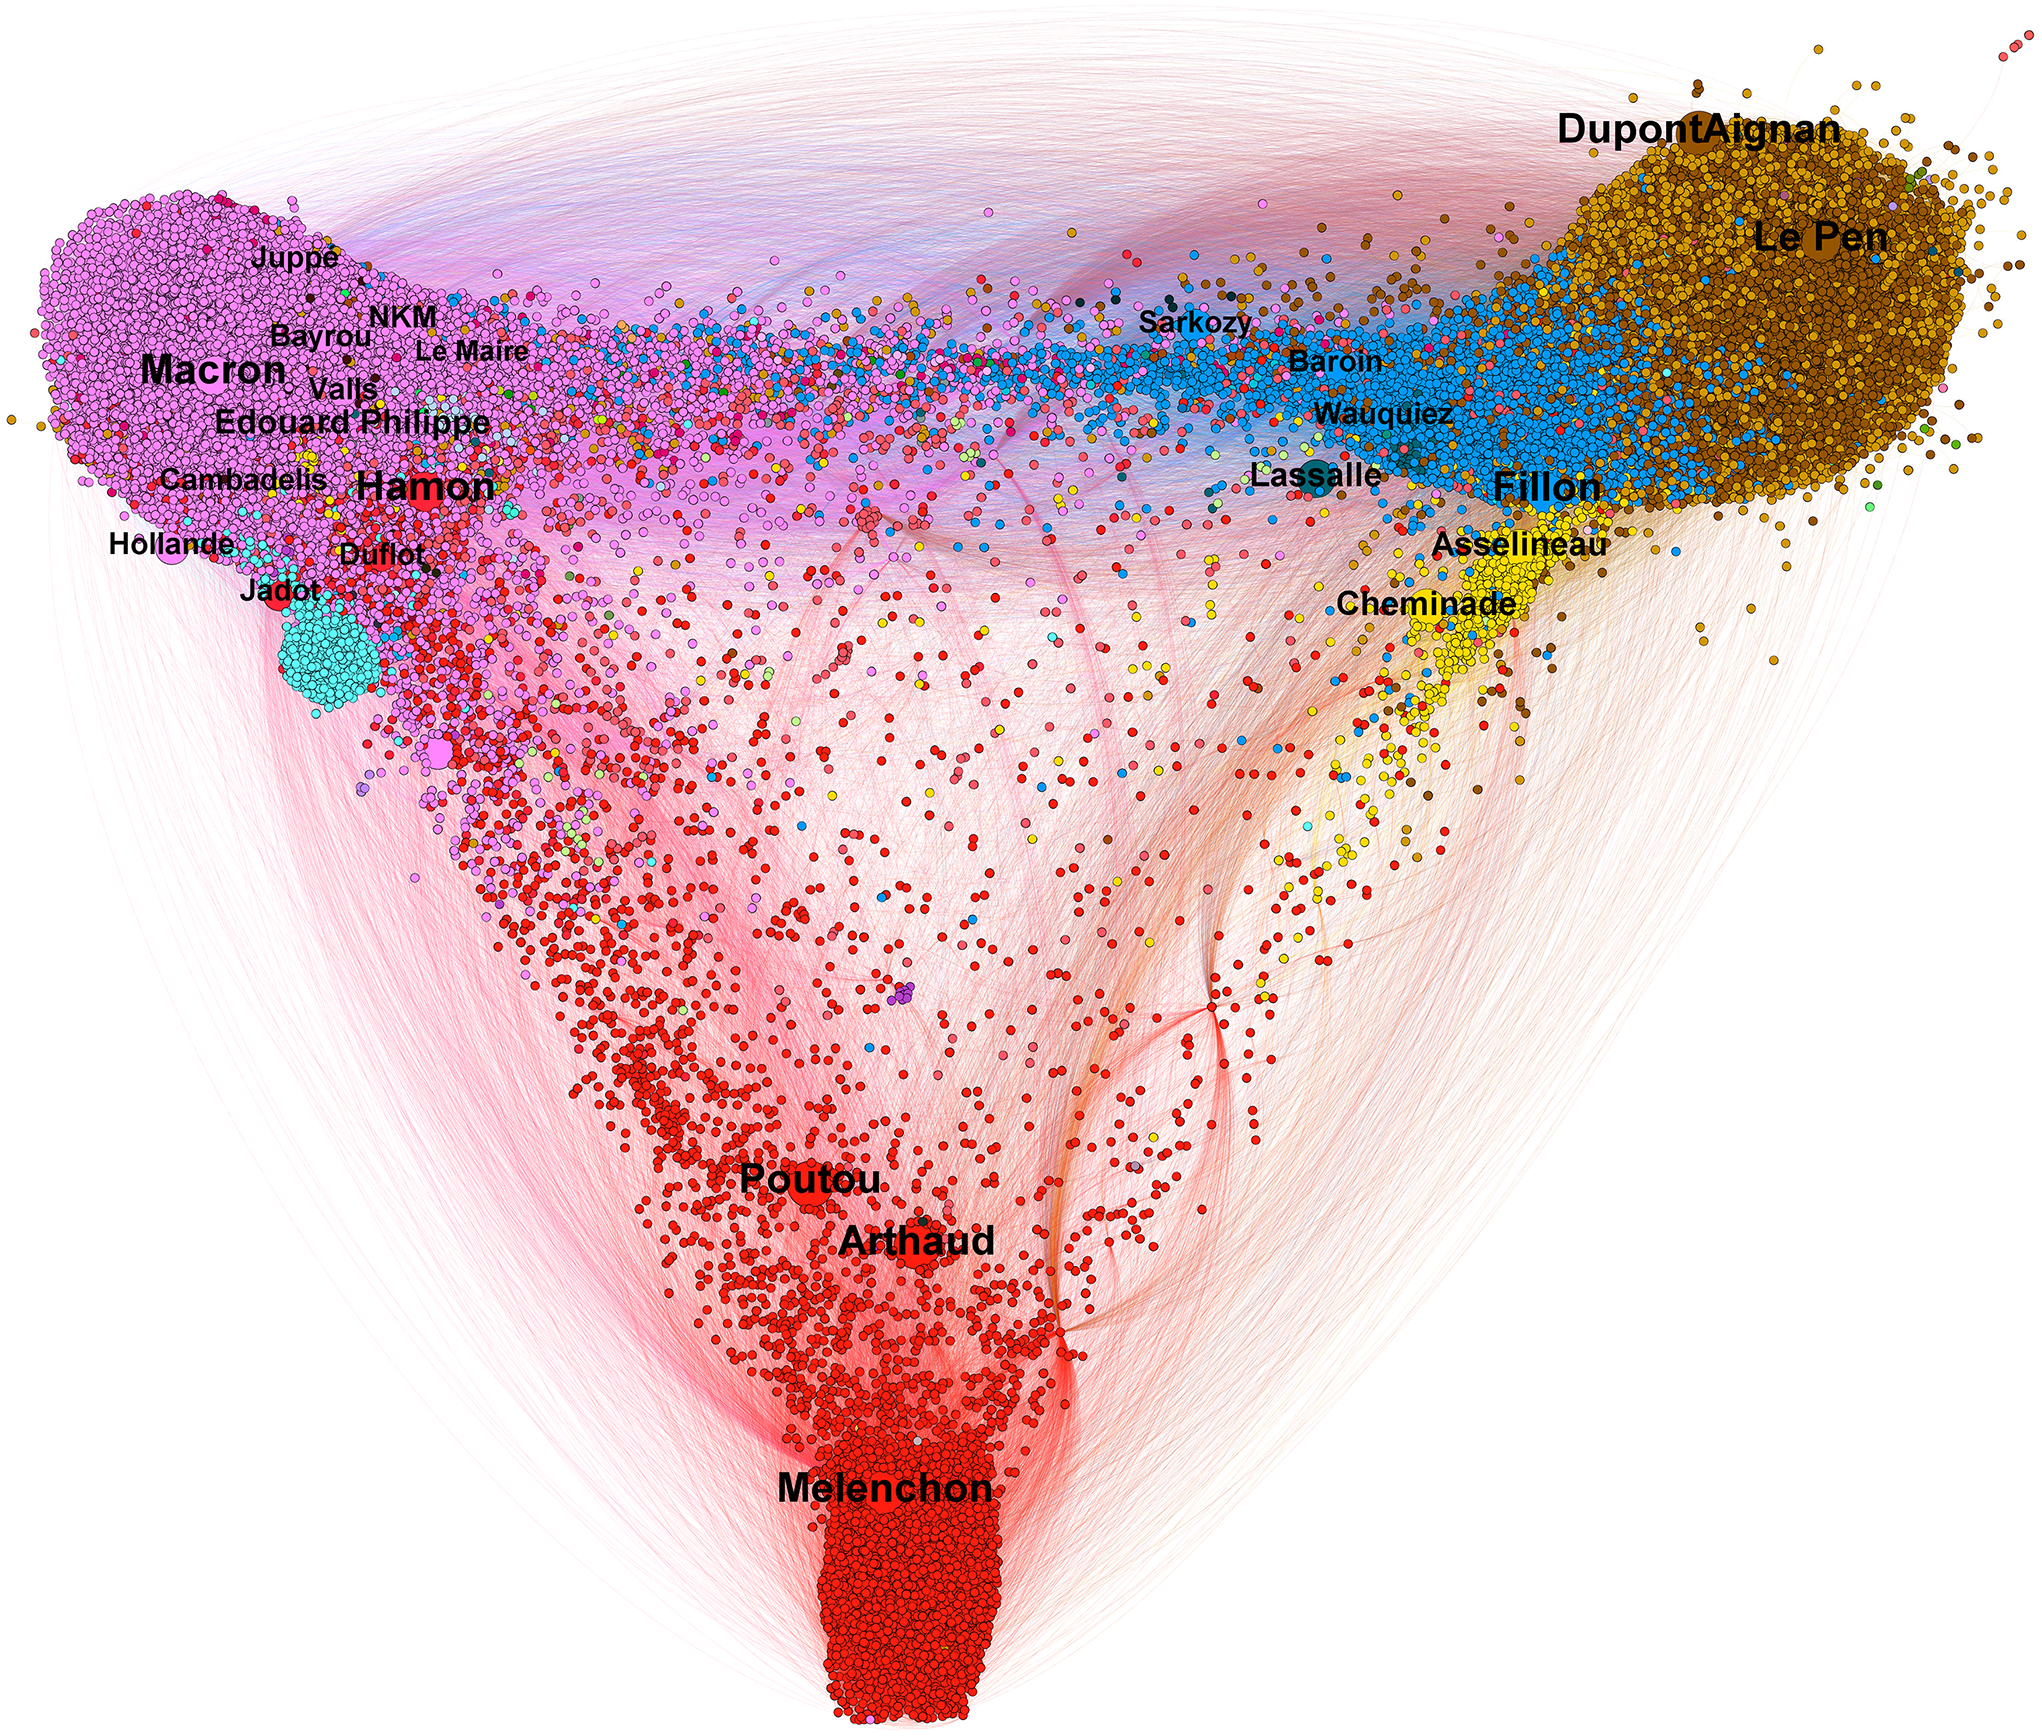
\includegraphics[width = 0.7\textwidth]{Chavalarias_fig_3.png}
        \caption{\small{Avant le second tour}}
      \end{figure}
\end{frame}

\begin{frame}
    \frametitle{IV) Quelques exemples d'usage des réseaux:}
    \begin{quotation}
        "Opinions and political communities vary together. Political campaigns involve reversals, bombshells, and reconfigurations of political support. (...) The main result of our study is that the automatic analysis of retweet patterns is able to measure, sometimes before the media can make any announcement, the changes taking place inside political communities in response to these events and, in some cases, in response to anticipated events. These changes can be of large magnitude in a very short period of time."
    \end{quotation}
    \begin{center}
        \small{Gaumont N., Panahi M., Chavalarias D., 2018, "Reconstruction of the socio-semantic dynamics of political activist Twitter networks—Method and application to the 2017 French presidential election", in \emph{PLoS ONE}, 13(9).}
    \end{center}
\end{frame}

\begin{frame}
    \frametitle{IV) Quelques exemples d'usage des réseaux:}
    \begin{itemize}
        \item Gaumont, Panahi, Chavalarias (2018): Étudient les réseaux socio-sémantiques politiques du twitter francophone pendant l'élection présidentielle française de 2017.
        \item Se focalisent sur les retweet de comptes politiques, et en infèrent une appartenance politique.
        \item Ils étudient la manière dont la structure du réseau de diffusion sur twitter évoluent durant toute la campagne. Ils traitent donc de l'aspect évolutif et longitudinal des réseaux.
    \end{itemize}
\end{frame}

\begin{frame}
    \frametitle{Conclusion:}
    \begin{itemize}
        \item Les réseaux sont une manière de représenter les structures relationnelles émergentes du monde social.
        \item Ce que vous pouvez dire de la structure du réseau dépends de vos choix méthodologiques: qui vous étudiez, quelles interactions, dans quel contexte?
        \item Il y a différentes manières d'étudier les réseaux. Plusieurs techniques de modélisation reposant sur diverses sous-structures existent.
    \end{itemize}
\end{frame}

\end{document}